\chapter{Τομή ευθείας-τετραέδρου}
\label{chapter:algs}
\section{Σημειολογία}
\subsection{Δεδομένα}
\label{chapter:alginput}
\noindent Στους αλγόριθμους που θα παρουσιαστούν στο παρόν κείμενο τα γεωμετρικά αντικείμενα (η ευθεία και το τετράεδρο) τα οποία ελέγχονται για την ύπαρξη τομής αναπαριστώνται ως εξής:

\emph{Ευθεία:} Η ευθεία στο συγκεκριμένο πρόβλημα είναι μια γραμμή άπειρου μήκους με συγκεκριμένη διεύθυνση και φορά. Η φορά της ευθείας επηρεάζει τα αποτελέσματα του αλγόριθμου, όπως θα προσδιοριστεί παρακάτω. Η ευθεία αναπαρίσταται από ένα σημείο $P$ επί αυτής και το διάνυσμα διεύθυνσής της, $L$. Στον κώδικα της υλοποίησης τα $P$ και $L$ είναι αντικείμενα που αντιπροσωπεύουν τριδιάστατα διανύσματα.  

\emph{Τετράεδρο:} Το τετράεδρο αναπαρίσταται από τις συντεταγμένες των τεσσάρων κορυφών του: $V_0,V_1,V_2,V_3$. Οι θέσεις των τεσσάρων κορυφών αντιπροσωπεύονται στον κώδικα της υλοποίησης από τριδιάστατα διανύσματα, παρομοίως με τα $P$ και $L$. Οι τέσσερις έδρες του τετραέδρου, $F_0,F_1,F_2,F_3,$ αριθμούνται με τον αριθμό της απέναντί τους κορυφής, ως εξής:

\begin{eqnarray*}
F_3 (V_0,V_1,V_2)\\	
F_2 (V_1,V_0,V_3)\\	
F_1 (V_2,V_3,V_0)\\		
F_0 (V_3,V_2,V_1)
\end{eqnarray*}
Στην περιγραφή του αλγόριθμου οι κορυφές της κάθε έδρας ονομάζονται ως εξής:\\
\begin{equation*}
 V^i_n
\end{equation*}
Όπου $i$ ο αριθμός της έδρας στην οποία ανήκει η κορυφή και $n$ ο αριθμός της κορυφής σε αυτή την έδρα, με την σειρά με την οποία παρατέθηκαν στην λίστα των εδρών. Για παράδειγμα, η κορυφή $V^3_0$  είναι η πρώτη  κορυφή της $F_3$, η $V_0$. Παρομοίως, οι ακμές της κάθε έδρας ονομάζονται ως εξής:

\begin{equation*}
e^i_k
\end{equation*}
Όπου $i$ ο αριθμός της έδρας στην οποία ανήκει η ακμή και $k$ ο αριθμός της απέναντί της κορυφής. Με αυτό τον τρόπο οι ακμές κατανέμονται ως εξής:

\begin{eqnarray*}
e^i_0 ({V^i_1 V^i_2})\\
e^i_1 ({V^i_2 V^i_0})\\	
e^i_2 ({V^i_0 V^i_1})		
\end{eqnarray*}
Για παράδειγμα, η ακμή $e^3_1$ ξεκινά από την κορυφή $V^3_2$  και καταλήγει στην $V^3_0$.\\

Οι αλγόριθμοι που θα παρουσιαστούν λειτουργούν με την παραδοχή ότι το τετράεδρο είναι προσανατολισμένο με τέτοιο τρόπο έτσι ώστε το κανονικό διάνυσμα κάθε έδρας $F_i$ να έχει τέτοια φορά  ώστε να απομακρύνεται από την αντίστοιχη κορυφή $V_i$. Ο προσανατολισμός του τετραέδρου είναι σημαντικός καθώς χρησιμοποιείται σε συσχετισμό με την φορά της ευθείας για να προσδιορίσει αν ένα σημείο τομής με την ευθεία είναι σημείο εισόδου ή εξόδου. Η διάκριση μεταξύ των σημείων εισόδου και εξόδου αναλύεται περαιτέρω στην ενότητα \ref{chapter:algs_pluck}.

\subsection{Ζητούμενα}
\label{chapter:algoutput}
\noindent Για κάθε ζεύγος ευθείας-τετραέδρου μπορεί να υπάρχει ή να μην υπάρχει τομή. Αν υπάρχει τομή, υπάρχουν τρεις περιπτώσεις, όπως φαίνονται στο σχήμα \ref{fig1}:

\begin{enumerate}
\item Η ευθεία τέμνει το τετράεδρο, άρα υπάρχουν δύο διακριτά σημεία $P_{enter}$ και $P_{leave}$ στα οποία η ευθεία εισέρχεται σε και εξέρχεται από το τετράεδρο αντίστοιχα.  

\item Η ευθεία τέμνει κάποια ακμή του τετραέδρου, άρα τα σημεία $P_{enter}$ και $P_{leave}$ ταυτίζονται.

\item Η ευθεία εφάπτεται σε κάποια έδρα του τετραέδρου, άρα υπάρχουν άπειρα σημεία τομής. Το σημείο στο οποίο η ευθεία εισέρχεται στην έδρα λογίζεται ως  $P_{enter}$ και αυτό από το οποίο εξέρχεται ως $P_{leave}$. 
\end{enumerate}
\pagebreak

\begin{figure}[t]
\center{ 
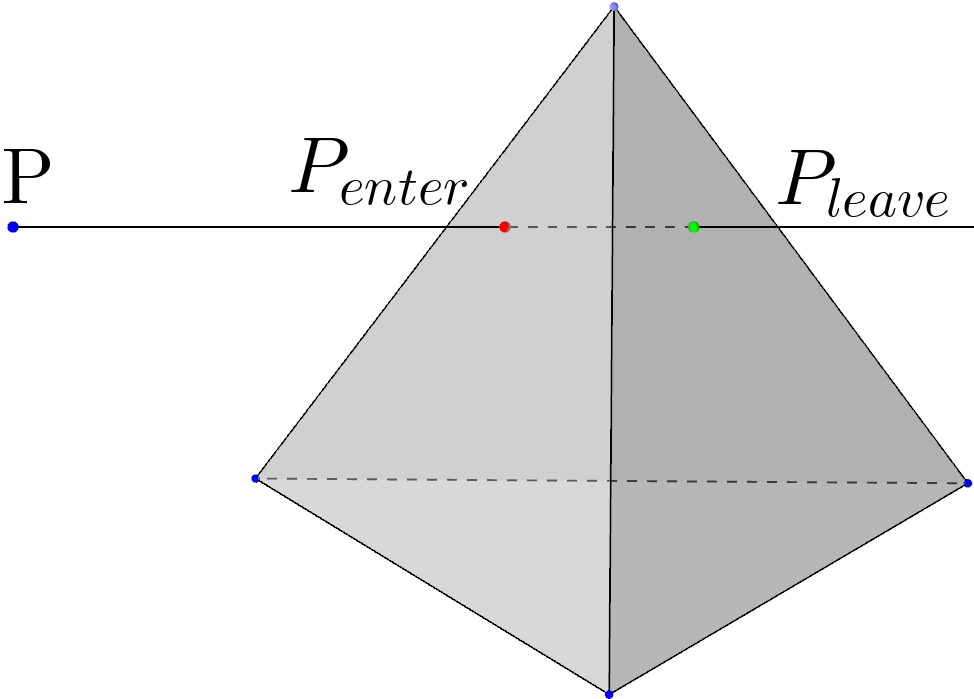
\includegraphics[scale=0.25]{graphics/raytetrarel0.png}
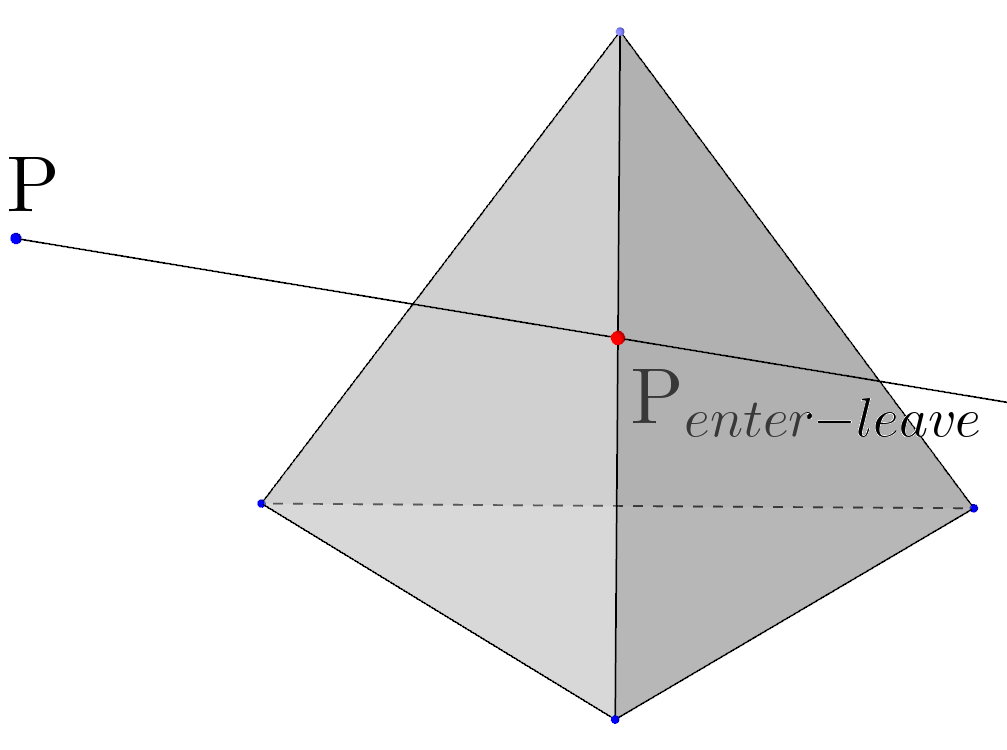
\includegraphics[scale=0.25]{graphics/raytetrarel1.png}
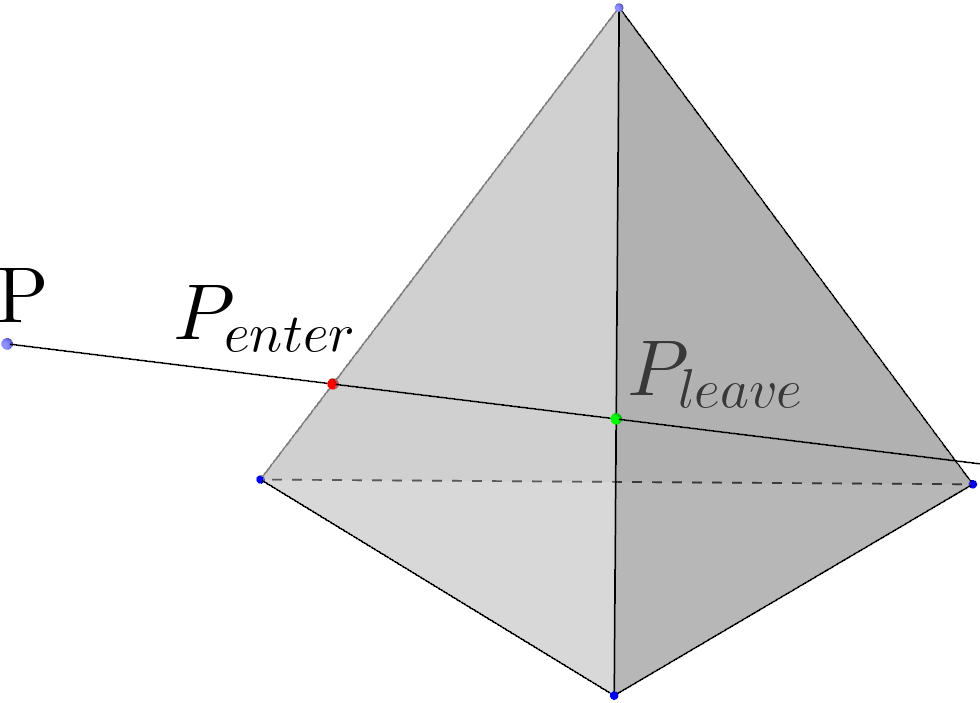
\includegraphics[scale=0.25]{graphics/raytetrarel2.png}}

\caption{Παραδείγματα των τριών περιπτώσεων τομής ευθείας-τετραέδρου.}
\label{fig1}
\end{figure}

Για κάθε τεμνόμενο ζεύγος ευθείας-τετραέδρου ο αλγόριθμος απαιτείται να υπολογίζει:

\begin{enumerate}
\item Τις καρτεσιανές συντεταγμένες των σημείων εισόδου και εξόδου, $P_{enter}$ και $P_{leave}$.  

\item Τις βαρυκεντρικές συντεταγμένες των σημείων εισόδου και εξόδου σε σχέση με τις έδρες ($F_{enter}$,$F_{leave}$) στις οποίες βρίσκονται. Συμβολίζονται ως $u^{enter}_1$,$u^{enter}_2$ και $u^{leave}_1$,$u^{leave}_2$. Για τις συντεταγμένες αυτές ισχύει ότι:

\begin{equation*}
P_k = (1 - u^k_1 - u^k_2)V^k_0 + u^k_1 V^k_1 + u^k_2 V^k_2
\end{equation*}
όπου $k= \text{enter} \text{ ή } \text{leave}$.
	
\item Τις παραμετρικές αποστάσεις $t_{enter}$ και $t_{leave}$ από το σημείο P το οποίο χρησιμοποιούμε για την αναπαράσταση της ευθείας. Για τις αποστάσεις αυτές ισχύει η σχέση:

\begin{equation*}
P_k = P +t_k L
\end{equation*}
όπου $k= \text{enter} \text{ ή } \text{leave}$.
\end{enumerate}
\pagebreak
\section{Αλγόριθμοι}
\label{chapter:algs_general}
\noindent  Στα πλαίσια της εργασίας αυτής δημιουργήθηκαν υλοποιημένες εκδόσεις δύο διαφορετικών αλγορίθμων. Οι δύο αυτοί αλγόριθμοι έχουν την ίδια βασική δομή. Ελέγχεται η ύπαρξη τομής μεταξύ της ευθείας και κάθε έδρας του τετραέδρου ξεχωριστά. Έτσι, ο έλεγχος τομής ευθείας-τετραέδρου αναλύεται σε τέσσερις ελέγχους τομής μεταξύ ευθείας και τριγώνου. Η διαφορά μεταξύ των δύο αλγορίθμων είναι η μέθοδος ελέγχου τομής ευθείας-τριγώνου που χρησιμοποιούν. Ο πρώτος βασίζεται στον έλεγχο τομής ευθείας-τριγώνου με συντεταγμένες Plücker που παρουσιάζεται στο ~\cite{PlatisTheoharis03}. Ο δεύτερος βασίζεται στον έλεγχο με χρήση μεικτού γινομένου τριών διανυσμάτων που αναφέρεται στο ~\cite{ericson2005real}.

Στην συνέχεια της ενότητας αυτής παρουσιάζονται οι δύο αυτές μέθοδοι ελέγχου τομής ευθείας-τριγώνου, το κοινό αλγοριθμικό πλαίσιο μέσω του οποίου συντίθεται ο έλεγχος τομής ευθείας-τετραέδρου και οι βελτιστοποιήσεις που επιδέχεται το πλαίσιο αυτό. 

\subsection{Τομή ευθείας-τριγώνου με συντεταγμένες Plücker}
\label{chapter:algs_pluck}
\noindent  Το σύστημα συντεταγμένων Plücker, που εισήχθη από τον Julius Plücker τον 19ο αιώνα\cite{plücker1828analytisch}, παρέχει μια μέθοδο ανάθεσης ομογενών συντεταγμένων σε κατευθυνόμενες ευθείες στον τριδιάστατο χώρο\cite{EricksonPlucker}. Στο σύστημα αυτό κάθε τέτοια ευθεία βρίσκεται σε 1-προς-1 αντιστοιχία με ένα εξαδιάστατο  διάνυσμα. Δεδομένης μια ευθείας $r$ η οποία ορίζεται από ένα σημείο $P$ και ένα διάνυσμα διεύθυνσης $L$, οι συντεταγμένες Plücker αυτής δίδονται από το διάνυσμα:

\begin{equation}
 \pi_r = \{L : L \times P ) = \{U_r : V_r\}		
\label{eq:plucker} 
\end{equation}

Μία από τις ιδιότητες των συντεταγμένων Plücker είναι ιδιαίτερα σημαντική για τους σκοπούς της εργασίας αυτής. Δεδομένων δύο ευθειών $r$ και $s$, το πρόσημο του αντιμετατεθημένου εσωτερικού γινομένου (permuted inner product) της σχέσης:

\begin{equation}
\pi_r \odot \pi_s = U_r \cdot V_s + U_s \cdot V_r	
\label{eq:permuted} 
\end{equation}
υποδεικνύει τον σχετικό προσανατολισμό των δύο ευθειών στο χώρο. Η έννοια του σχετικού προσανατολισμού δύο ευθειών στο χώρο επεξηγείται στο σχήμα \ref{fig:2}. 
\begin{figure}[b!]
1.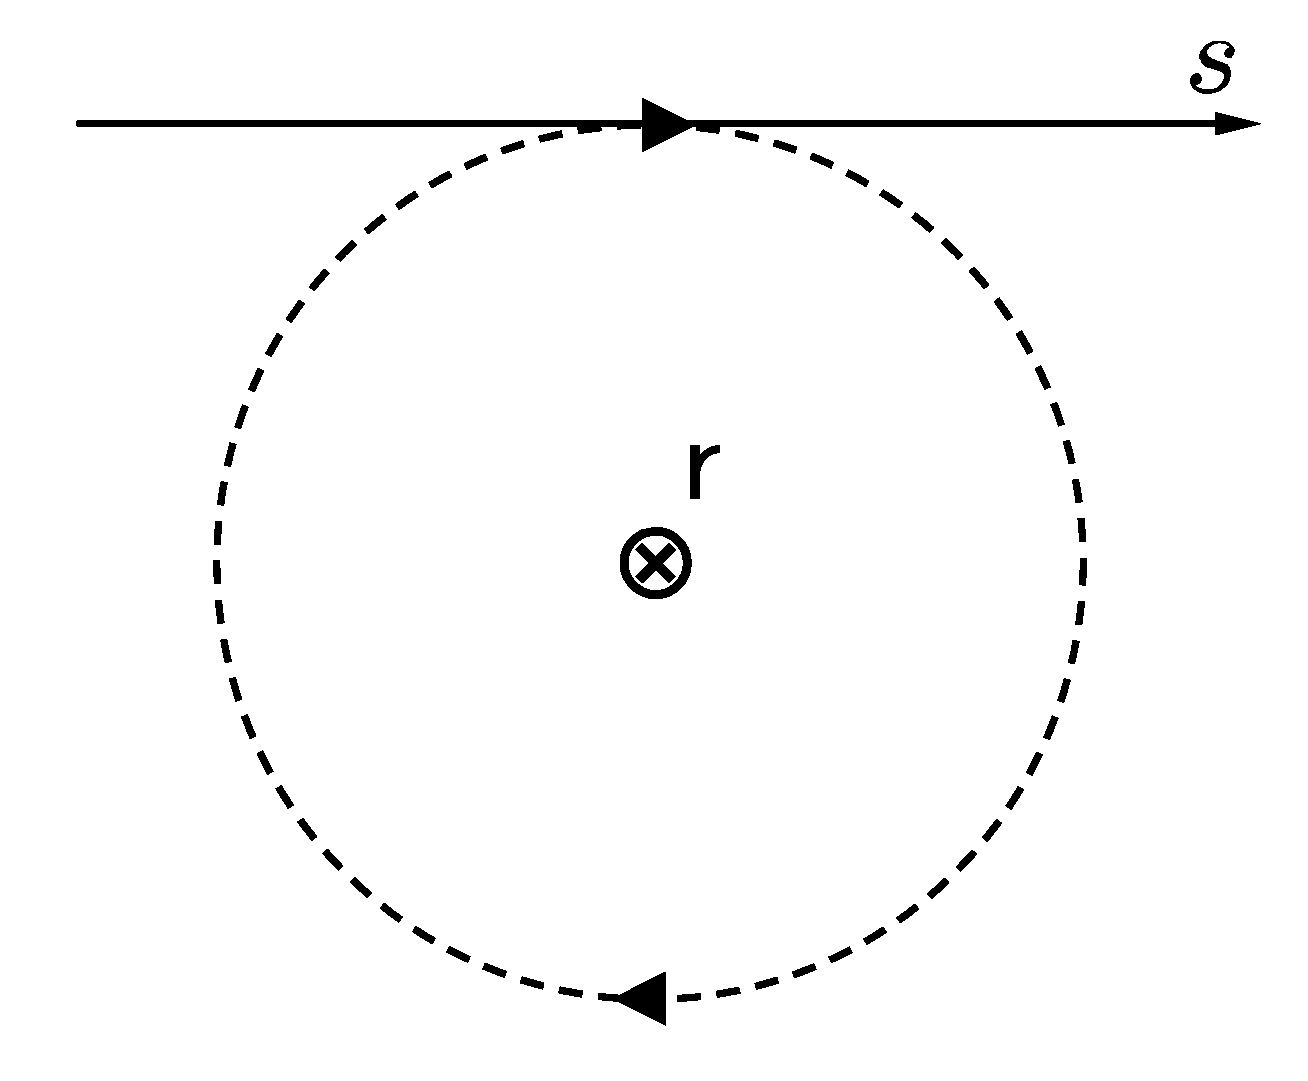
\includegraphics[scale=0.2]{graphics/orientations_cw.eps}
2.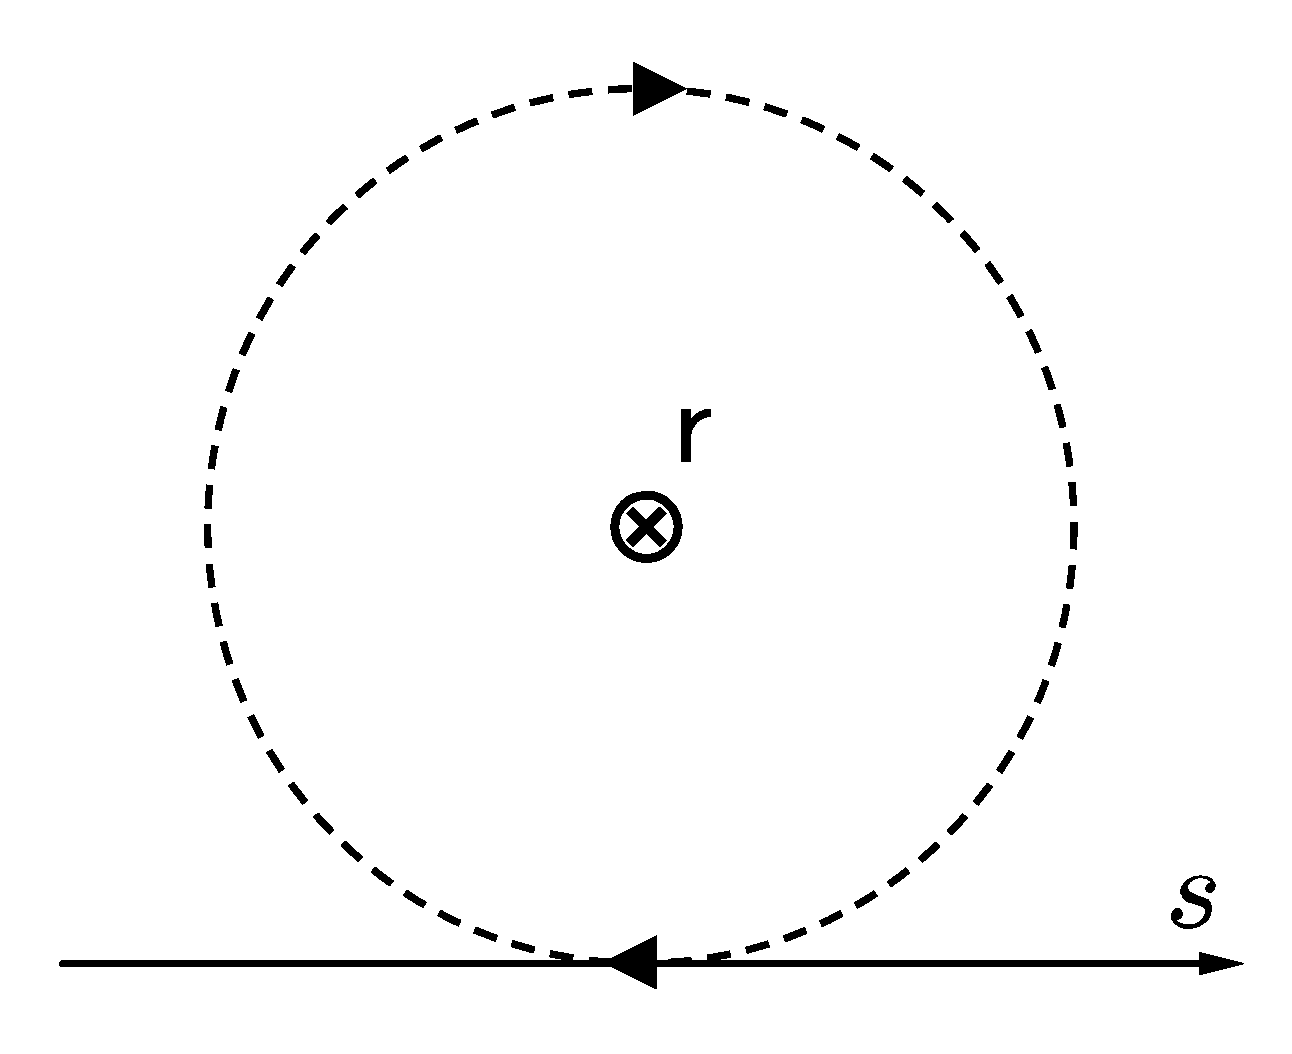
\includegraphics[scale=0.2]{graphics/orientations_ccw.eps}
3.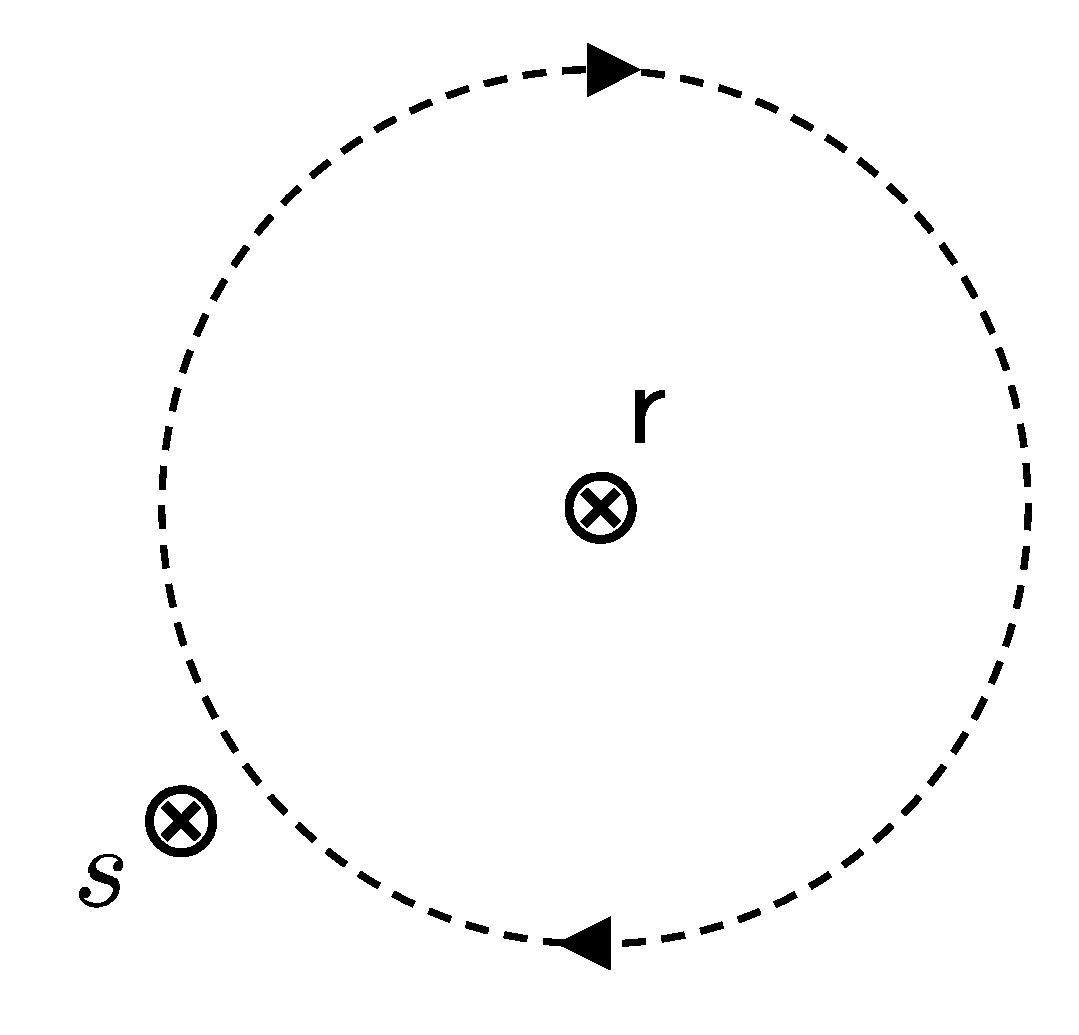
\includegraphics[scale=0.2]{graphics/orientations_parallel.eps}
\vspace*{20pt}\centering{4.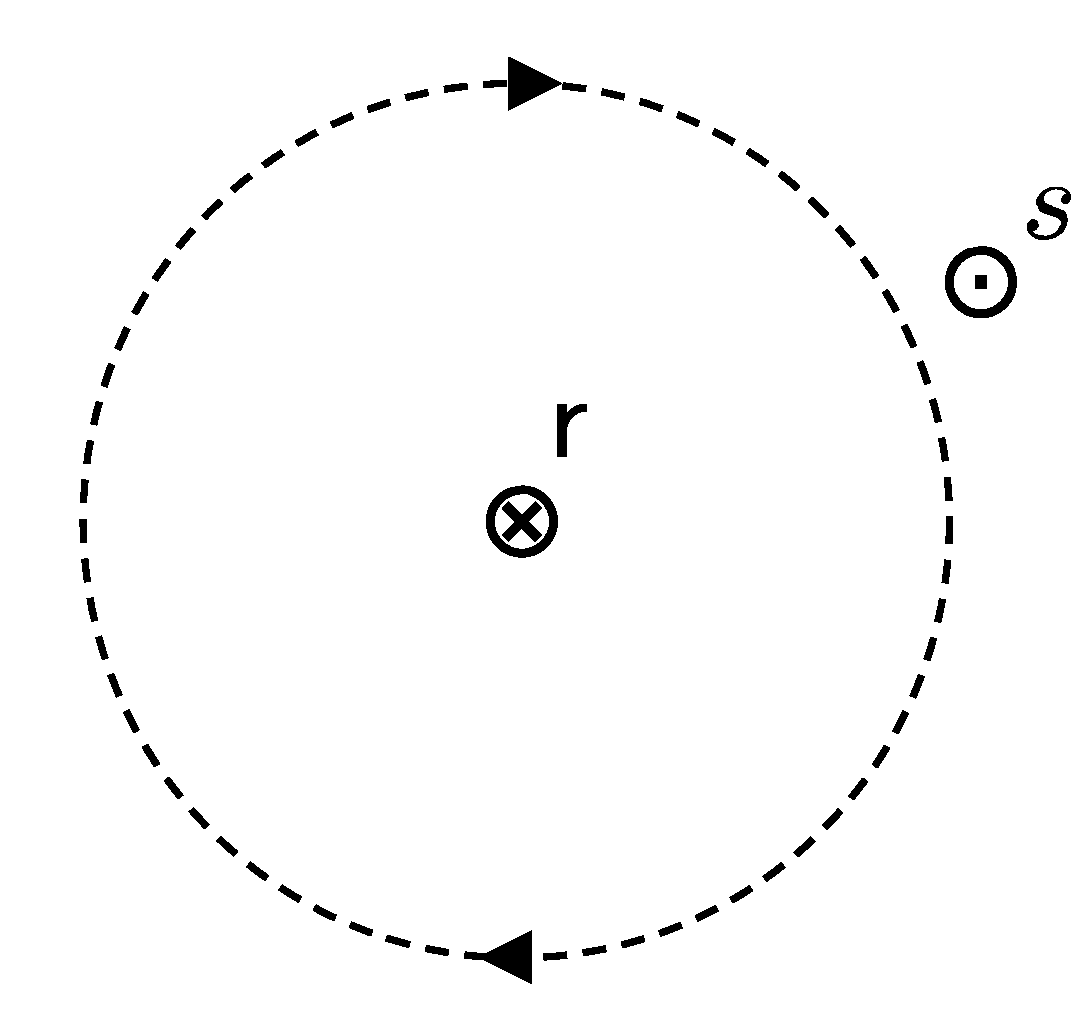
\includegraphics[scale=0.2]{graphics/orientations_antiparallel.eps}
5.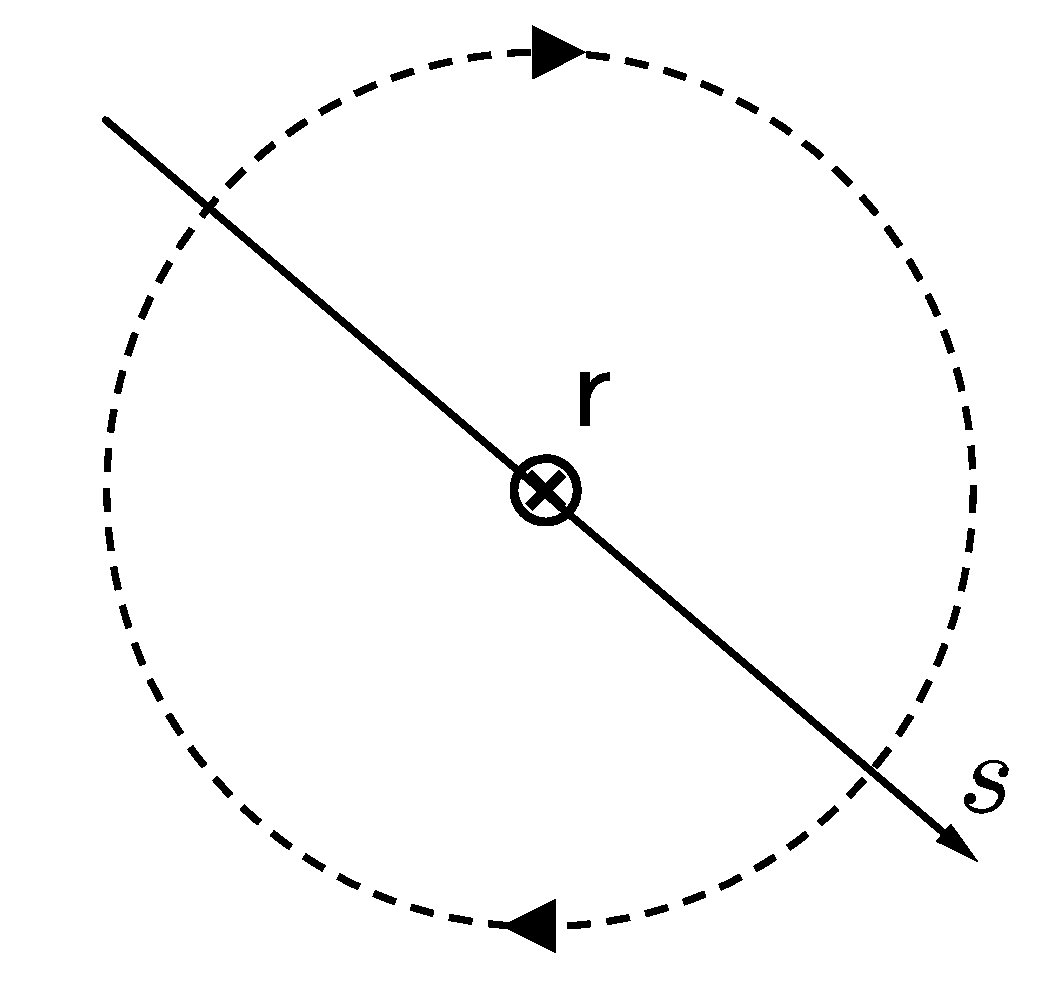
\includegraphics[scale=0.2]{graphics/orientations_intersect.eps}}
\captionsetup{singlelinecheck=off}
\caption[Σχετικός προσανατολισμός δύο κατευθυνόμενων ευθειών]{Σχετικός προσανατολισμός δύο κατευθυνόμενων ευθειών $r$ και  $s$ στον χώρο.  H ευθεία $r$ είναι κάθετη στο επίπεδο της σελίδας και την παρατηρούμε κοιτάζοντας κατά την κατεύθυνσή της. Οι περιπτώσεις είναι οι εξής:\begin{enumerate}\item H $s$ στρέφεται με φορά ρολογιού σε σχέση με την $r$.\item H $s$ στρέφεται  με φορά  αντίθετη του ρολογιού σε σχέση με την $r$.\item H $s$ είναι παράλληλη στην $r$.\item H $s$ είναι αντιπαράλληλη στην $r$.\item H $s$ τέμνει την $r$.\end{enumerate}}
\label{fig:2}
\end{figure} 

Το πρόσημο του αντιμετατεθημένου εσωτερικού γινομένου της σχέσης \eqref{eq:permuted} αντιστοιχεί στον σχετικό προσανατολισμό των $r$ και $s$ ως εξής: 

\begin{enumerate}

\item
$\pi_r \odot \pi_s > 0\iff$Η $s$ στρέφεται με φορά ρολογιού σε σχέση με την $r$.
\item
$\pi_r \odot \pi_s < 0\iff$Η $s$ στρέφεται με φορά αντίθετη του ρολογιού σε σχέση με την $r$.
\nolinebreak\item 
$\pi_r \odot \pi_s = 0\iff$Η $s$ τέμνει ή είναι παράλληλη στην $r$.\\
\label{linecrit}
\end{enumerate}

Με βάση την ιδιότητα αυτή μπορεί να αναπτυχθεί η εξής μέθοδος για τον έλεγχο τομής ευθείας-τριγώνου:\\

Έστω ευθεία $r$ και τρίγωνο $\Delta(V_0,V_1,V_2)$ με ακμές $e_0(V_1V_2)$, $e_1(V_2V_0)$, $e_2(V_0V_1)$. Ισχύει ότι η $r$ τέμνει το $\Delta$ \textbf{αν και μόνο αν} έχει τον ίδιο σχετικό προσανατολισμό και με τις τρεις ακμές $e_0,e_1,e_2$ ή αν τέμνει το πολύ δύο από αυτές. Άρα, ισχύουν τα ακόλουθα:

\begin{enumerate}
\item
Η $r$ τέμνει (εισερχόμενη) το $\Delta$ αν: \begin{equation*}\pi_r \odot \pi_{e_{i}} \geq 0\; \forall\; i\in \{0,1,2\}\; KAI \; \exists \,j : \pi_r \odot \pi_{e_{j}} \neq 0\end{equation*}
\item
Η $r$ τέμνει (εξερχόμενη) το $\Delta$ αν:\begin{equation*}\pi_r \odot \pi_{e_{i}} \leq 0\; \forall\; i\in \{0,1,2\}\;  KAI \; \exists \,j : \pi_r \odot \pi_{e_{j}} \neq 0 \end{equation*}
\item
Η $r$ είναι συνεπίπεδη με το $\Delta$ αν: \begin{equation}\pi_r \odot \pi_{e_{i}}= 0 \;\forall\; i\in \{0,1,2\}\; \label{eq:crit}  \end{equation}
\end{enumerate}

Στις περιπτώσεις 1 και 2 οι τιμές των αντιμετατεθημένων εσωτερικών γινομένων $\pi_r \odot \pi_{e_{i}}$ παρέχουν άμεσα τις βαρυκεντρικές συντεταγμένες του σημείου τομής $P_k$ ως προς τις κορυφές $V_{0,1,2}$, όπως αποδεικνύεται στο ~\cite{JonesIntersect}. Έστω:\\
\begin{equation}w^k_i=\pi_r \odot \pi_{e_{i}}
\label{eq:bary1} 
\end{equation}
H συνισταμένη $u^k_i$ των βαρυκεντρικών συντεταγμένων του σημείου τομής $P_k$ ως προς την κορυφή $V_i$ ισούται με:
\begin{equation}
u^k_i = \frac{w^k_i}{\displaystyle\sum_{i=0}^{3} w^k_i}  \qquad
\label{eq:bary2} 
\end{equation}
Οι καρτεσιανές συντεταγμένες του σημείου $P_k$ μπορούν να βρεθούν ως εξής:

\begin{equation}
P_k = u^k_0 V_0 + u^k_1 V_1 + u^k_2 V_2
\label{eq:cart} 
\end{equation}
Επιπλέον, η παραμετρική απόσταση από το σημείο $P$ επί της ευθείας μπορεί να υπολογιστεί λύνοντας ως προς $t_k$ την σχέση

\begin{equation}
P_k = P + t_k L
\label{eq:para} 
\end{equation}
για οποιαδήποτε μη-μηδενική συνισταμένη των συντεταγμένων του διανύσματος διεύθυνσης $L$.

\subsection{Τομή ευθείας-τριγώνου με μεικτό γινόμενο}
\label{chapter:stpalg}
\noindent  Η προσέγγιση αυτή βασίζεται σε μια εναλλακτική μέθοδο υπολογισμού του σχετικού προσανατολισμού δύο ευθειών που παρουσιάζεται στα ~\cite{ericson2005real} και ~\cite{ericson2007blog} από τον C. Ericson. Η μέθοδος αυτή απορρέει από την διαπίστωση ότι, στα πλαίσια της εύρεσης του σχετικού προσανατολισμού δύο κατευθυνόμενων ευθύγραμμων τμημάτων (και κατ' επέκταση ευθειών), το αντιμετατεθημένο εσωτερικό γινόμενο της σχέσης \eqref{eq:permuted} είναι μαθηματικώς ισοδύναμο με το μεικτό γινόμενο τριών διανυσμάτων τα οποία αντιπροσωπεύουν τα δύο ευθύγραμμα τμήματα.

Έστω δύο κατευθυνόμενα ευθύγραμμα τμήματα $AB$ και $CD$. Ορίζονται τα διανύσματα $\vec{p} = B -A$, $\vec{q} = C -A$, $\vec{r} = D -A$ όπως φαίνονται στο σχήμα ~\ref{fig3}.
\begin{figure}[t!]
\centering{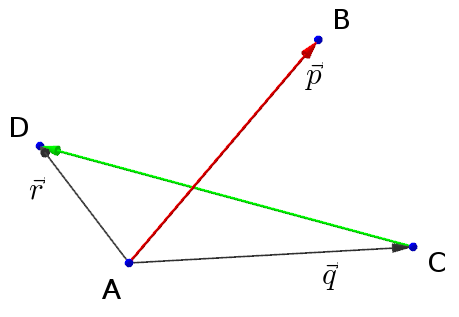
\includegraphics[scale=0.6]{graphics/stp.png}}
\caption{Αντιστοιχία των διανυσμάτων p,q,r με τα ευθύγραμμα τμήματα AB και CD. }
\label{fig3}
\end{figure}
\begin{figure}[b!]
\centering{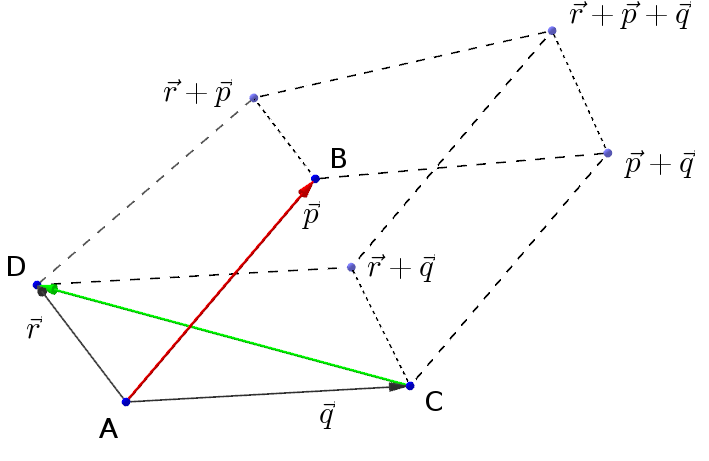
\includegraphics[scale=0.6]{graphics/stp_volume.png}}
\caption{Το παραλληλεπίπεδο που ορίζεται από τα διανύσματα p,q,r.}
\label{fig4}
\end{figure}
Η ποσότητα $\vec{p} \cdot (\vec{q} \times \vec{r})$ ονομάζεται  μεικτό γινόμενο των $\vec{p},\vec{q},\vec{r}$ και μπορεί να συμβολιστεί ως $[p q r]$. Το μεικτό γινόμενο έχει την ιδιότητα να είναι αμετάβλητο για οποιοδήποτε πιθανή κυκλική μετάθεση των στοιχείων του, δηλαδή ισχύει:

\begin{equation}
[p q r] = [r p q] = [q r p]
 \label{eq:circular}
\end{equation}

Οι μη κυκλικές μεταθέσεις προκύπτουν με απλή αλλαγή του προσήμου:

\begin{equation}
[p q r] = -[q p r]\;\;,\;\;[q p r] = -[r p q] \;\;\text{κ.ο.κ.}
\label{eq:noncircular}
\end{equation}

Το μεικτό γινόμενο $[p q r]$ μπορεί να χρησιμοποιηθεί για την εύρεση του σχετικού προσανατολισμού των $AB$ και $CD$ στον χώρο ακριβώς όπως το αντιμετατεθημένο εσωτερικό γινόμενο των συντεταγμένων Plücker της σχέσης \eqref{eq:permuted}. Απόδειξη της ισοδυναμίας των δύο μεθόδων υπάρχει στην δημοσίευση \cite{kensler:06:triangle}. Η ισοδυναμία αυτή προκύπτει από το γεγονός ότι τα δύο αυτά μεγέθη αντιστοιχούν στην ίδια γεωμετρική ποσότητα, τον προσημασμένο όγκο του παραλληλεπιπέδου ο οποίος ορίζεται από τα τρία αυτά διανύσματα (σχήμα \ref{fig4}). Ο όγκος αυτός είναι προσημασμένος καθώς εξαρτάται από τον σχετικό προσανατολισμό των $p$,$q$,$r$ και κατ' επέκταση των $AB$,$CD$.

Στην περίπτωση που εξετάζουμε ισχύει ότι:

\begin{enumerate}
\item
 Αν $[p q r] > 0\iff$Το $CD$ στρέφεται με φορά ρολογιού σε σχέση με το $AB$.
\item
Αν $[p q r] < 0\iff$Το $CD$ στρέφεται με φορά αντίθετη του ρολογιού σε σχέση με το $AB$.
\item
Αν $[p q r] = 0\iff$ Το $CD$ τέμνει ή είναι παράλληλο προς το $AB$.\\
\end{enumerate}
Ο έλεγχος τομής ευθείας-τριγώνου που παρουσιάστηκε στην προηγούμενη ενότητα μπορεί να πραγματοποιηθεί ισοδύναμα με την χρήση μεικτού γινομένου. Στην περίπτωση αυτή το ευθύγραμμο τμήμα $AB$ αντιστοιχεί σε αυτό που ορίζεται από τα σημεία $P$ και $L$ (με φορά από το $P$ προς το $L$) και το $CD$ στην εκάστοτε ακμή του τριγώνου (με την φορά της ακμής). Για παράδειγμα, στον έλεγχο σχετικού προσανατολισμού της ευθείας με την ακμή $e_0(V_1V_2)$  τα αντίστοιχα διανύσματα $p$,$q$,$r$ είναι τα εξής: $p=L$, $q=V_0-P$, $ r=V_1-P$. Αντίστοιχα προσαρμόζεται ο έλεγχος των υπόλοιπων ακμών.

\subsection{Βασικός αλγόριθμος τομής ευθείας-τετραέδρου}
\label{chapter:raytetraint}
\noindent  Με βάση τον έλεγχο τομής ευθείας-τριγώνου που αναφέρθηκε μπορεί να αναπτυχθεί εύκολα ένας βασικός αλγόριθμος τομής ευθείας-τετραέδρου. Ο αλγόριθμος ελέγχει κάθε έδρα του τετραέδρου με την σειρά με βάση τα κριτήρια της παράστασης \eqref{eq:crit}. Aν κάποια από τις έδρες διαπιστωθεί οτι είναι η έδρα εισόδου ($F_{enter}$) ή η έδρα εξόδου ($F_{leave}$) τότε ο αντίστοιχος έλεγχος δεν πραγματοποιείται για τις υπόλοιπες έδρες. 

Στην συνέχεια του κειμένου, όταν γίνεται αναφορά στην έδρα $F_i$ του τετραέδρου θα συμβολίζονται ως $\pi^i_j$ οι συντεταγμένες Plücker της ακμής $e^i_j$  και ως $\sigma^i_j$ το πρόσημο του αντιμετατεθημένου εσωτερικού γινομένου $\pi_r \odot \pi^i_j$ για την δεδομένη ευθεία $r$ ή του ισοδύναμου μεικτού γινομένου. Επίσης, ως ${e^i_j}_{(\alpha)}$ και ${e^i_j}_{(\beta)}$ συμβολίζονται η αρχική και τελική (σύμφωνα με την φορά) κορυφή της έδρας $e^i_j$. Ισχύει ότι:

\begin{equation}
\sigma^i_j =\text{sign}(\pi_r \odot \pi^i_j) = \text{sign}(\;[L({e^i_j}_{(\alpha)}-P)({e^i_j}_{(\beta)}-P)]\;)\\ 
\label{eq:sigmatostp} 
\end{equation}
\begin{equation}
\sigma^i_j =
\begin{cases}
 \;\; \;1,\;\text{αν}\,\pi_r \odot \pi^i_j>0\text{ ή, ισοδύναμα,} \;[L({e^i_j}_{(\alpha)}-P)({e^i_j}_{(\beta)}-P)]\;>0 \\
 \;\; \;0,\;\text{αν}\,\pi_r \odot \pi^i_j=0\text{ ή, ισοδύναμα,} \;[L({e^i_j}_{(\alpha)}-P)({e^i_j}_{(\beta)}-P)]\;=0 \\
 \; -1,\;\text{αν}\,\pi_r \odot \pi^i_j<0\text{ ή, ισοδύναμα,} \;[L ({e^i_j}_{(\alpha)}-P)({e^i_j}_{(\beta)}-P)]<0 \\
\end{cases}
\end{equation}

Ο αλγόριθμος εκφράζεται σε ψευδοκώδικα ως εξής:
\floatname{algorithm}{Αλγόριθμος}
\begin{algorithm}[H]
\caption{Ο βασικός αλγόριθμος Τομής Ευθείας-Τετραέδρου}
\label{segura0}
\begin{algorithmic}
\STATE $F_{enter} \gets nil$
\STATE $F_{leave} \gets nil$
\FOR{$ i = 3, 2, 1, 0$}
\STATE Υπολογισμός $\sigma^i_0$,$ \sigma^i_1$,$\sigma^i_2$
\IF{$ (( \sigma^i_0 \neq 0)$ \OR $( \sigma^i_1  \neq 0)$ \OR  $(\sigma^i_2  \neq 0))$}
\IF{ $((F_{enter} == nil)$ \AND $ \sigma^i_0 \geq 0)$ \AND $( \sigma^i_1 \geq 0)$ \AND $( \sigma^i_2 \geq 0))$}
\STATE$ F_{enter} \gets F_i$
\ELSIF {$((F_{leave} == nil)$ \AND $( \sigma^i_0 \leq 0)$ \AND  $(\sigma^i_1 \leq 0)$ \AND $(\sigma^i_2 \leq 0))$}
\STATE$ F_{leave} \gets F_i$
\ENDIF
\ENDIF
\ENDFOR
\end{algorithmic}
\end{algorithm}

Ο αλγόριθμος αυτός μπορεί επιπρόσθετα να χρησιμοποιηθεί  για τον υπολογισμό των βαρυκεντρικών συντεταγμένων χρησιμοποιώντας τις σχέσεις \eqref{eq:bary1} και \eqref{eq:bary2}. Ομοίως, οι σχέσεις \eqref{eq:cart}
και \eqref{eq:para} μπορούν να χρησιμοποιηθούν για τον υπολογισμό των καρτεσιανών συντεταγμένων του σημείου τομής και των παραμετρικών αποστάσεων από το $P$ αντίστοιχα. Επίσης μπορούν να εντοπιστούν εύκολα οι ειδικές περιπτώσεις στις οποίες η ευθεία εφάπτεται σε κάποια ακμή ή έδρα του τετραέδρου, καθώς στις περιπτώσεις αυτές ένα ή δύο από τα $\sigma^i_j$ για κάποια τιμή του $i$ ισούνται με 0.

Στην υλοποίηση η οποία έγινε στα πλαίσια της εργασίας, η βασική αυτή μορφή του αλγορίθμου ονομάζεται μορφή 0.  

\subsection{Βελτιστοποιήσεις}

\noindent Ο αλγόριθμος που παρουσιάστηκε στην ενότητα \ref{chapter:raytetraint} επιδέχεται πολλές βελτιστοποιήσεις. Οι βελτιστοποιήσεις αυτές προέρχονται από τρεις βασικές τροποποιήσεις του τρόπου λειτουργίας του αλγορίθμου:

\begin{itemize}
\item Την απαλοιφή των μη απαραίτητων ελέγχων.
\item Την επανάληψη χρήσης των ήδη υπολογισμένων ποσοτήτων για διαφορετικές έδρες του τετραέδρου.
\item Την αξιοποίηση των γεωμετρικών χαρακτηριστικών του προβλήματος.  
\end{itemize}

Οι βελτιστοποιήσεις που ακολουθούν βασίζονται στις πρώτες δύο τροποποιήσεις και προέρχονται από τις ενότητες 3.1 και 3.2 του \cite{PlatisTheoharis03}.

\begin{enumerate}
\item Ο αλγόριθμος μπορεί να τερματίσει άμεσα αν έχουν προσδιοριστεί τα $F_{enter}$ και $F_{leave}$ χωρίς να εξετάσει τις υπόλοιπες έδρες του τετραέδρου.
\item Μόνο τρεις από τις τέσσερις έδρες του τετραέδρου είναι απαραίτητο να ελεγχθούν. Αν και οι τρεις δεν τέμνονται από την ευθεία τότε είναι αδύνατον να τέμνεται η τέταρτη. Αν κάποια από τις τρεις τέμνεται τότε και η τέταρτη θα τέμνεται. Η τέταρτη έδρα θα είναι η $F_{enter}$ αν έχει ήδη βρεθεί η $F_{leave}$ ή η $F_{leave}$ αν έχει ήδη βρεθεί η $F_{enter}$. 
\item Κάθε ακμή του τετραέδρου ανήκει σε δύο διαφορετικές έδρες και διατρέχεται με αντίθετη φορά σε καθεμία από αυτές. Η τιμή του $\sigma$ χρειάζεται να υπολογιστεί μόνο μία φορά για κάθε ακμή. Το $\sigma$ της ακμής με τις ίδιες κορυφές και αντίθετη φορά προκύπτει με απλή αλλαγή του προσήμου του ήδη υπολογισμένου. Για παράδειγμα, η $e^3_2$ $(V_{0}V_{1})$ και η $e^2_2$ $(V_{1}V_{0})$ διαφέρουν μόνο κατά την φορά. Ισχύει ότι:
\begin{equation*}
\pi_r \odot \pi^3_2 = -(\pi_r \odot \pi^2_3)
\end{equation*}
\begin{equation*}
[L (V_1-P) (V_0-P)] = - [L (V_0-P) (V_1-P)]
\end{equation*}

Στην περίπτωση της χρήσης συντεταγμένων Plücker η ιδιότητα αυτή προκύπτει από τον ορισμό των συντεταγμένων Plücker και του αντιμετατεθημένου εσωτερικού γινομένου. Στην περίπτωση του μεικτού γινομένου προκύπτει από την σχέση \ref{eq:noncircular}.
\item Όταν έχει βρεθεί μία έδρα που τέμνεται από την ευθεία και απομένουν μόνο δύο έδρες προς έλεγχο είναι δυνατόν να προσδιοριστεί η άλλη τεμνόμενη έδρα πραγματοποιώντας μόνο ένα υποσύνολο των συγκρίσεων προσήμων που χρειάζονται στην γενική περίπτωση. Η επιλογή ανάμεσα στις δύο έδρες βασίζεται στο πρόσημο της κοινής τους ακμής. Για παράδειγμα, έστω ότι πρέπει να βρεθεί ποια από τις $F_1(V_2V_3V_0)$ και $F_0(V_3V_2V_1)$ είναι η $F_{leave}$. Αν $\pi_r \odot \pi_{V_2V_3} < 0$ τότε $F_{leave}$ είναι η $F_1$, αλλιώς είναι η $F_0$. Εξαίρεση αποτελεί η περίπτωση στην οποία όλα τα $\sigma^0_j$ είναι 0 οπότε ισχύει ότι $F_{leave}$ είναι η $F_1$. 
\item Στον βασικό αλγόριθμο ο έλεγχος κάθε έδρας του τετραέδρου περιλαμβάνει τον υπολογισμό και των τριών ποσοτήτων $\sigma^i_j$. Όμως, αν δύο από αυτές δεν έχουν το ίδιο πρόσημο τότε δεν είναι απαραίτητο να υπολογιστεί και να συγκριθεί η τρίτη. Η βελτιστοποίηση αυτή περιπλέκεται από το γεγονός ότι ένα ή δύο από τα $\sigma^i_j$ μπορεί να ισούνται με 0. Η βελτιστοποιημένη εκδοχή του έλεγχου για την έδρα $F_i$ είναι η εξής:

\floatname{algorithm}{Αλγόριθμος}
\begin{algorithm}[H]
\caption{Βελτιστοποίηση του ελέγχου έδρας}
\label{segura1inner}
\begin{algorithmic}
\STATE Υπολογισμός $\sigma^i_0$ και $\sigma^i_1$.
\STATE \{Έλεγχος ισότητας των $\sigma^i_0$ και $\sigma^i_1$ μεταξύ τους και με το 0. Αν διαφέρουν και είναι μη μηδενικά δεν υπάρχει τομή με αυτή την έδρα.\}
\IF{(($\sigma^i_0 == \sigma^i_1$ ) \OR ($\sigma^i_0 == 0$) \OR ($\sigma^i_1 == 0$))}

\STATE Υπολογισμός $\sigma^i_2$
\STATE \{Εύρεση του προσήμου $\sigma^i$ της έδρας. Το $\sigma^i$ είναι ίσο με το πρώτο από τα  $\sigma^i_0$ και $\sigma^i_1$ που είναι μη μηδενικό, ή το $\sigma^i_2$ αν και τα δύο είναι μηδενικά.\}

\STATE $\sigma^i =\gets \sigma^i_0$

\IF{($\sigma^i == 0$)}

\STATE $\sigma^i \gets \sigma^i_1$

\IF{($\sigma^i == 0$)}

\STATE $\sigma^i \gets \sigma^i_2$
\ENDIF
\ENDIF
\STATE \{Για να υπάρχει τομή πρέπει το $\sigma^i_2$ να έχει ίδιο πρόσημο με το $\sigma^i$, ή να είναι μηδενικό. Στην περίπτωση που το $\sigma^i$ είναι μηδενικό η ευθεία είναι συνεπίπεδη με την έδρα.\}

\IF{(($\sigma^i \neq 0$) \AND ($(\sigma^i_2 == \sigma^i $) \OR $(\sigma^i_2 == 0$)))}
\STATE \{Διάκριση μεταξύ έδρας εισόδου και εξόδου.\}
\IF {$(\sigma^i > 0$)}
\STATE $F_{enter} \gets F_i$
\ELSE
\STATE $F_{leave} \gets F_i$
\ENDIF
\ENDIF
\ENDIF
\end{algorithmic}
\end{algorithm}
   
\item Όταν βρεθεί μία έδρα η οποία τέμνεται από την ευθεία ο βελτιστοποιημένος έλεγχος που παρουσιάστηκε μπορεί να απλοποιηθεί περαιτέρω για τις έδρες που απομένουν. Οι ακμές της τεμνόμενης έδρας που είναι κοινές με τις υπόλοιπες έδρες έχουν γνωστό πρόσημο $\sigma$ (βλ. βελτιστοποίηση 3) και ο έλεγχος για τις υπόλοιπες ακμές απλοποιείται στο $\sigma^i_j \leq 0$ αν έχει βρεθεί η $F_{enter}$ ή $\sigma^i_j \geq 0$ αν έχει βρεθεί η $F_{leave}$.
\end{enumerate}

Στον κώδικα της υλοποίησης η εκδοχή του αλγορίθμου τομής ευθείας-τετραέδρου η οποία ενσωματώνει τις βελτιστοποιήσεις που αναφέρθηκαν ονομάζεται μορφή 1.

Η τελευταία βελτιστοποίηση προέρχεται από την τρίτη πιθανή τροποποίηση του αλγορίθμου: Την αξιοποίηση των γεωμετρικών χαρακτηριστικών του προβλήματος. Έστω ότι η πρώτη έδρα του τετραέδρου που ελέγχεται είναι η $F_3(V_0V_1V_2)$. Αν τέμνεται από την ευθεία, ο αλγόριθμος συνεχίζει όπως  ακριβώς έχει περιγραφεί. Αν όχι, τότε η ευθεία πρέπει να τέμνει το επίπεδο στο οποίο ανήκει η $F_3$ σε μία από τις έξι περιοχές τις οποίες ορίζουν οι ευθείες οι οποίες περιέχουν τις τρεις ακμές της έδρας $F_3$ (σχήμα \ref{fig5}). Οι περιοχές αυτές αντιστοιχούν σε διαφορετικά εύρη βαρυκεντρικών συντεταγμένων στο επίπεδο αυτό σε σχέση με τα $V_0,V_1,V_2$. Ανάλογα με την περιοχή και με την διεύθυνση της ευθείας υπάρχει μόνο μία πιθανή έδρα του τετραέδρου που μπορεί να είναι η $F_{enter}$ ή η $F_{leave}$ (κατά περίπτωση).
Αν αυτή βρεθεί ότι δεν τέμνεται τότε είναι αδύνατον να υπάρχει σημείο τομής για αυτό το ζεύγος ευθείας-τετραέδρου.

Στο παράδειγμά μας αν η ευθεία τέμνει «εισερχόμενη» το επίπεδο στην περιοχή E τότε μπορεί να εισέρχεται στο τετράεδρο μόνο στην έδρα $F_1(V_2V_3V_0)$, ενώ αν «εισέρχεται» στην περιοχή Α τότε η μόνη πιθανή $F_{leave}$ είναι η $F_0(V_3V_2V_1)$. Για να γίνει πιο κατανοητή η διάκριση μεταξύ των περιπτώσεων όπου η ευθεία «εισέρχεται» και αυτών που «εξέρχεται» στο επίπεδο διευκρινίζεται ότι η ευθεία θεωρείται «εισερχόμενη» όταν ισχύει:

\begin{equation*}
\displaystyle\sum_{j=0}^{2}(\pi_r \odot \pi^3_j) > 0
\end{equation*}
Ο έλεγχος αυτός είναι ισοδύναμος με τον έλεγχο $L \cdot N < 0$, όπου Ν το κάθετο διάνυσμα της έδρας που ελέγχεται.

\begin{figure}[h!]
\centering{
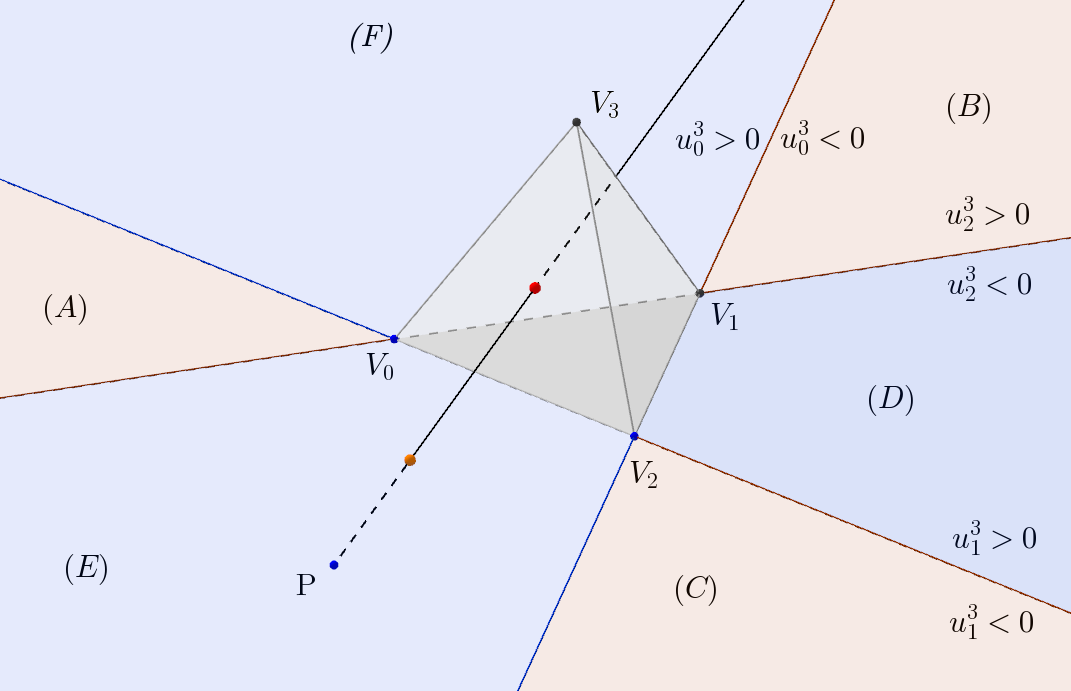
\includegraphics[scale=0.5]{graphics/alg2areas.png}}
\caption{Ο διαχωρισμός του επιπέδου της $F_3(V_0V_1V_2)$ σε περιοχές με βάση τις ευθείες των ακμών της. Στο παράδειγμα αυτό η ευθεία τέμνει το επίπεδο στην περιοχή $E$, άρα η έδρα που πρέπει να εξεταστεί από τον αλγόριθμο είναι η $F_1(V_2V_3V_0)$.}
\label{fig5}
\end{figure}
Η αντιστοιχία των περιοχών του επιπέδου που τέμνει η ευθεία ως «εισερχόμενη» ή «εξερχόμενη» και των εδρών τις οποίες δύναται να τέμνει είναι η εξής:

\begin{center}
  \begin{tabular}{ | c || c || c | }
    \hline
    Περιοχή & Εισερχόμενη & Εξερχόμενη \\ \hline \hline
    A & $F_0 = F_{leave}$ & $F_0 = F_{enter}$ \\ \hline
    B & $F_1 = F_{leave}$ & $F_1 = F_{enter}$ \\ \hline
    C & $F_2 = F_{leave}$ & $F_2 = F_{enter}$ \\ \hline
    D & $F_0 = F_{enter}$ & $F_0 = F_{leave}$ \\ \hline
    E & $F_1 = F_{enter}$ & $F_1 = F_{leave}$ \\ \hline
    F & $F_2 = F_{enter}$ & $F_2 = F_{leave}$ \\ \hline
  \end{tabular}
\end{center}

Η βελτιστοποίηση αυτή έχει ενσωματωθεί στην μορφή 2 της υλοποίησης. 



   
